\documentclass{standalone}
\usepackage{tikz}
\usepackage{ctex,siunitx}
\setCJKmainfont{Noto Serif CJK SC}
\usepackage{tkz-euclide}
\usepackage{amsmath}
\usetikzlibrary{patterns, calc}
\usetikzlibrary {decorations.pathmorphing, decorations.pathreplacing, decorations.shapes,}

\begin{document}
\small
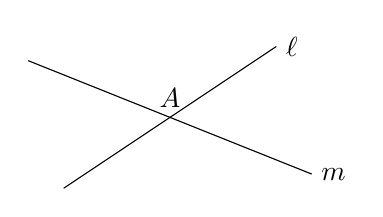
\begin{tikzpicture}[>=stealth,scale=0.9]
  \tkzSetUpPoint[fill=black]
  % \useasboundingbox(-1,-0.75)rectangle(3.7,1.4);
  \draw (-2,.8)--(2,-.8)node[right]{$m$};
  \draw (-1.5,-1)--(1.5,1)node[right]{$\ell$};
  \node at (0,0)[above]{$A$};
\end{tikzpicture}
\end{document}